\documentclass[border=6pt]{standalone}
\usepackage{ctex,amsmath,amssymb,tikz}
\usetikzlibrary{arrows.meta,positioning,patterns,calc,decorations.pathreplacing}
\begin{document}
% 截面法示意：固定 z，再把截面投影到 xy 平面。
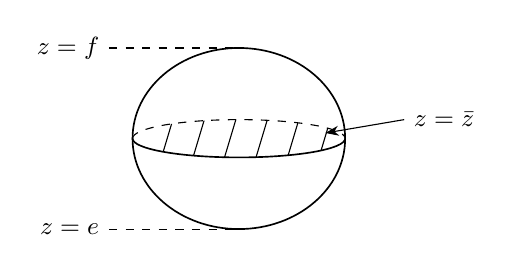
\begin{tikzpicture}[>=Stealth,font=\small]
  \draw[line width=.6pt] (0,0) ellipse[x radius=1.35,y radius=1.15];
  \draw[dashed] (-1.35,0) arc[start angle=180,end angle=0,x radius=1.35,y radius=.24];
  \draw[line width=.6pt] (-1.35,0) arc[start angle=180,end angle=360,x radius=1.35,y radius=.24];
  \begin{scope}
    \clip (0,0) ellipse[x radius=1.35,y radius=.24];
    \foreach \s in {-1,-.6,-.2,.2,.6,1}
      \draw[thin] (\s,-.3) -- ({\s+.18},.3);
  \end{scope}
  \draw[dashed] (-1.65,1.15) -- (0,1.15);
  \draw[dashed] (-1.65,-1.15) -- (0,-1.15);
  \node[left] at (-1.65,1.15) {$z=f$};
  \node[left] at (-1.65,-1.15) {$z=e$};
  \draw[->] (2.1,.24) -- (1.1,.07);
  \node[right] at (2.1,.24) {$z=\bar z$};
\end{tikzpicture}

\end{document}